% =========================================================
% Chapter 6 — Verification
% =========================================================

\section{Simulation Strategy}

The firmware was verified at two levels before hardware testing: unit simulation of individual modules and a system-level integration testbench. All unit tests were written using the cocotb framework~\cite{cocotb} with Icarus Verilog~\cite{icarus} as the simulator, following the same runner pattern throughout the project. The exception is the sensor control FSM, which is written in VHDL and was tested with a dedicated VHDL testbench under ModelSim~\cite{modelsim}.

Cocotb was chosen to allow test logic to be written in Python, reducing testbench development ime and making the tests readable without requiring HDL expertise. ModelSim was retained for the VHDL sensor control FSM, where native VHDL simulation was preferred. A consequence of this split is that two simulators are used across the project; a unified approach using cocotb with ModelSim for all modules was not pursued due to licensing constraints.

The cocotb unit tests target individual module sin isolation and do not require any Xilinx IP simulation models, since none of the modules under test instantiate IP cores directly.

A system-level testbench was initially developed in ModelSim before the cocotb framework was adopted. It used behavioural stub models to replace the Xilinx IP cores --- the XADC Wizard, the MMCM clock generator, and the TMDS output buffers --- so tha the surrounding logic could be simulated without a depedency on Xilinx simulation libraries. This approach was superseded by the cocotb unit tests, which test each module in isoaltion and avoid the complexity of a full system-level simulation environment.

\section{UART Loopback Tests}

The UART transmitter and receiver modules were verified together using a loopback testbench (\texttt{sim/cocotb/uart}). The test wrapper connects the transmitter output directly tot he receiver input so that every byte sent by the transmitter is received and checked.

The simulation uses an accelerated clock (10~MHz) and a proportionally faster baud rate (1~Mbit/s), 10 clock cycles per bit) to keep simulation time practical. Five test cases were run:

\begin{itemize}
  \item \textbf{Single byte} - transmit 0x55 (alternating bits, maximum transition density) and verify the received value matches.
  \item \textbf{All zeros} - transmit 0x00 (long low period, tests start-bit detection).
  \item \textbf{All ones} - transmit 0xFF (long high period after the stop bit).
  \item \textbf{Sequential bytes} - transmit 0x00 through 0x0F in sequence and verify each arrives in order with no dropped bytes.
  \item \textbf{Idle line} - verify that the TX line is held high when no transmission is in progress.
\end{itemize}

All five tests passed, confirming correct framing (start bit, 8 data bits, stop bit) and bit ordering across the full range of byte values.

% TODO: insert waveform showing loopback of 0x55 — TX line, RX line,
%       data_valid pulse, and received byte value.
%       Capture from: sim/cocotb/uart/sim_build/dump.vcd

\section{UART Register Interface Tests}

The register interface module (\texttt{uart\_reg\_if.sv}) was verified with eight test cases in \texttt{sim/cocotb/uart\_reg\_if/}. The test wrapper instantiates a host transmitter (to inject frames into the DUT) and a host receiver (to capture the DUT response), along with a 256-entry read memory that can be pre-loaded by the test.

The protocol under test uses four-byte frames: a write frame is \\
\texttt{0xAA~<addr>~<data>~0x55} and a read frame is \texttt{0xBB~<addr>~0x55}, producing the response \texttt{0xCC~<addr>~<data>~0x55}.

The test cases cover:

\begin{itemize}
  \item \textbf{Write frame} - verify that \texttt{write\_en} pulses with the correct address and data after a valid write frame.
  \item \textbf{Bad write footer} - a frame with an incorrect footer byte must not assert \texttt{write\_en}.
  \item \textbf{Full read response} - a read frame must produce exactly four response bytes in the correct order: header, address echo, data, footer.
  \item \textbf{Response byte count} - verify that no spurious fifth byte appears after a valid read response.
  \item \textbf{Multiple addresses} - read three different addresses in sequence and verify each response contains the correct pre-loaded value.
  \item \textbf{Idle after write} - verify that the DUT returns to IDLE after a completed write and accepts a second frame immediately.
  \item \textbf{Bad read footer} - a read frame with an incorrect footer must produce no response.
\end{itemize}

A regression test was included to guard against a previously observed timing defect. Before the fix, consecutive transmit states in the DUT fired within a one-cycle window before the UART transmitter asserted \texttt{tx\_busy}, causing only two of the four response bytes to be sent. The fix uses a one-cycle delayed copy of \texttt{tx\_busy} (\texttt{tx\_busy\_d}) as the readiness gate. The regression test verifies that all four bytes of the response are present and correctly ordered.

The tests confimed that the protocol framing is correctly decoded, that malformed frames are silenty rejected wihtout side effects, and that the read response contains exactly four bytes in the correct order. The regression test specifically confirmed that the \texttt{tx\_busy\_d} fix resolved the race condition - without it, only two of the four response bytes were transmitted.
% TODO: insert waveform showing a complete read transaction:
%       BB <addr> 55 sent, CC <addr> <data> 55 received.
%       Capture from: sim/cocotb/uart_reg_if/sim_build/dump.vcd

\section{Control Register Tests}

The register file module (\texttt{control\_regs.sv}) was verified with ten test cases in \texttt{sim/cocotb/control\_regs/}. The tests exercise both local (buttons/switch) and remote (UART) control modes and verify that the arbitration between them is correct.

Key test cases include:

\begin{itemize}
    \item \textbf{Reset defaults} - after reset, \texttt{exposure\_us} = 100~$\mu$s, \texttt{dwell\_us} = 100~$\mu$s, \texttt{reset\_us} = 10~$\mu$s, \texttt{cds\_delay\_us} = 2~$\mu$s.
    \item \textbf{Remote register writes} - in remote mode, writing \texttt{EXP\_LO}/\texttt{EXP\_HI} updates \texttt{exposure\_us} correctly as a 16-bit little-endian value.
    \item \textbf{Button ignored in remote mode} - a \texttt{delay\_up} pulse in remote mode must not change \texttt{exposure\_us}.
    \item \textbf{Local button increment/ddecrement} - in local mode, \texttt{delay\_up} and \texttt{delay\_down} change \texttt{exposure\_us} by exactly 10~$\mu$s per pulse.
    \item \textbf{Switch pass-through} - in local mode, \texttt{sw\_cds\_enable}, \texttt{sw\_photosense}, and \texttt{sw\_invert\_pol} drive the corresponding outputs directly.
    \item \textbf{Write blocked outside remote mode} - a write to any register other than \texttt{CTRL} (0x00) is silently ignored when \texttt{remote\_mode} is not set.
    \item \textbf{Start pulse edge detect} - in remote mode, setting \texttt{CTRL[0]} produces a \texttt{start\_pulse} for exactly one clock cycle; it does not remain high.
    \item \textbf{MODE register outputs} - writing 0x1E to MODE sets \texttt{invert\_pol}~=~1, \texttt{disp\_gain}~=~3, \texttt{photosense\_mode}~=~1, \texttt{read\_mode}~=~0.
\end{itemize}

The tests confirmed that local and remote control modes are correctly arbitrated, that register writes outside remote mode are blocked, that button inputs are ignored in remote mode, and that the start pulse generates a single-cycle edge rather than a sustained signal.

% TODO: (optional) waveform showing start_pulse edge detect —
%       CTRL[0] rising edge produces exactly one-cycle pulse.

\section{Clock Domain Crossing Tests}

The CDC synchroniser (\texttt{cdc\_adc\_sync.sv} was verified with six test cases in \texttt{sim/cocotb/cdc\_adc\_sync/}. Two independent clocks drive the source (100~MHz, 10~ns period) and destination (74.25~MHz, 13.47~ns period) domains.

\begin{itemize}
    \item \textbf{Single transfer} - a \texttt{data\_valid} pulse with sensor value 0xABC and temperature value 0x123 must appear at the destination outputs after the synchroniser latency.
    \item \textbf{Zero and maximim values} - 0x000 and 0xFFF must transfer without corruption.
    \item \textbf{Sequential transfers} - four consecutive samples must each arrive with the correct values, with sufficient inter-sample spacing to allow the handshake to complete.
    \item \textbf{Output stability} - after a transfer completes, the destination outputs must hold their values indefinitely without a new \texttt{data\_valid} pulse.
    \item \textbf{Latency bound} - the transfer must complete within six \texttt{clk\_dst} cycles of the \texttt{data\_valid} pulse (three synchronizer stages plus one output register stage, with margin).
\end{itemize}

The tests confirmed that 12-bit values transfer correctly across the clock boundary without corruption, that the output holds its value between transfers, and that the synchronizer latency stays within the expected bound of six \texttt{clk\_dst} cycles - consistent with the three-stage synchroniser design described in Chapter~5.

% TODO: (optional) waveform showing toggle_src flip, 3-FF synchroniser
%       chain, and data capture at destination.
%       Capture from: sim/cocotb/cdc_adc_sync/sim_build/dump.vcd

\section{Sensor FSM Unit Tests}

The sensor control FSM (\texttt{sensor\_ctrl.vhd}) was verified with five cocotb test cases in \texttt{sim/cocotb/sensor\_ctrl/}, run under ModelSim via a Mafefile runner. The clock period is set to 13.47~ns (74.25~MHz) and timing parameters are set to small values to keep simulation time manageable.

\begin{itemize}
    \item \textbf{Reset idles} - after hardware reset, the FSM remains in IDLE and all control outputs (\texttt{nRES}, \texttt{nTX} are deasserted.
    \item \textbf{Reset phase} - a start pulse moves the FSM to RESET, \texttt{nRES} goes low, and the FSM holds RESET for the configured \texttt{reset\_us} duration.
    \item \textbf{Full frame scan} - with CDS disabled, the FSM transitions IDLE~$\to$~RESET~$\to$~INTEGRATE~$\to$~READOUT and produces \texttt{pixel\_step} pulses at the correct addresses for all 64 pixels of the default 8$\times$8 array.
    \item \textbf{CDS phase} - with \texttt{cds\_enable} asserted, the FSM inserts the CDS state between RESET and INTEGRATE and holds it for \texttt{cds\_delay\_us}.
    \item \textbf{Single-pixel mode} - with \texttt{read\_mode} asserted, the FSM enters SINGLE\_PIXEL after INTEGRATE and continuously asserts the selected pixel address.
\end{itemize}

% TODO: insert GTKWave waveform from sim/cocotb/sensor_ctrl/ showing
%       full frame scan: nRES, nTX, AX, AY, pixel_step across one
%       complete cycle. Run: cd sim/cocotb/sensor_ctrl && make
%       then open the VCD in GTKWave to export the figure.

\section{Hardware Bring-Up}

After simulation, the design was synthesised and implemented in Vivado~2024.2 and programmed onto the Nexys Video board. Bring-up proceeded in three stages: control signal verification, readout timing verification, and pixel data acquisition.

\subsection{Control Signal Verification}

The sensor control signals on the PMOD~JA header were probed with an oscilloscope to verify that the FPGA produced the correct waveforms. Figures~\ref{fig:ctrl_test1} and~\ref{fig:ctrl_test2} show the \texttt{nRES} and \texttt{nTX} signals during the reset and integration phases. The measured pulse widths were compared against the register values configured via the Python GUI.

% ---- FIGURE: control signal test 1 ----
% Suggested caption: "nRES and nTX waveforms during the RESET and
%   INTEGRATE phases. nRES is held low for reset_us, then nTX goes low
%   for the duration of exposure_us."
% Files: figures/scope/ctrl_signal_test_1_scope/print_00.png
%        figures/scope/ctrl_signal_test_1_scope/print_01.png
\begin{figure}[h]
  \centering
  % 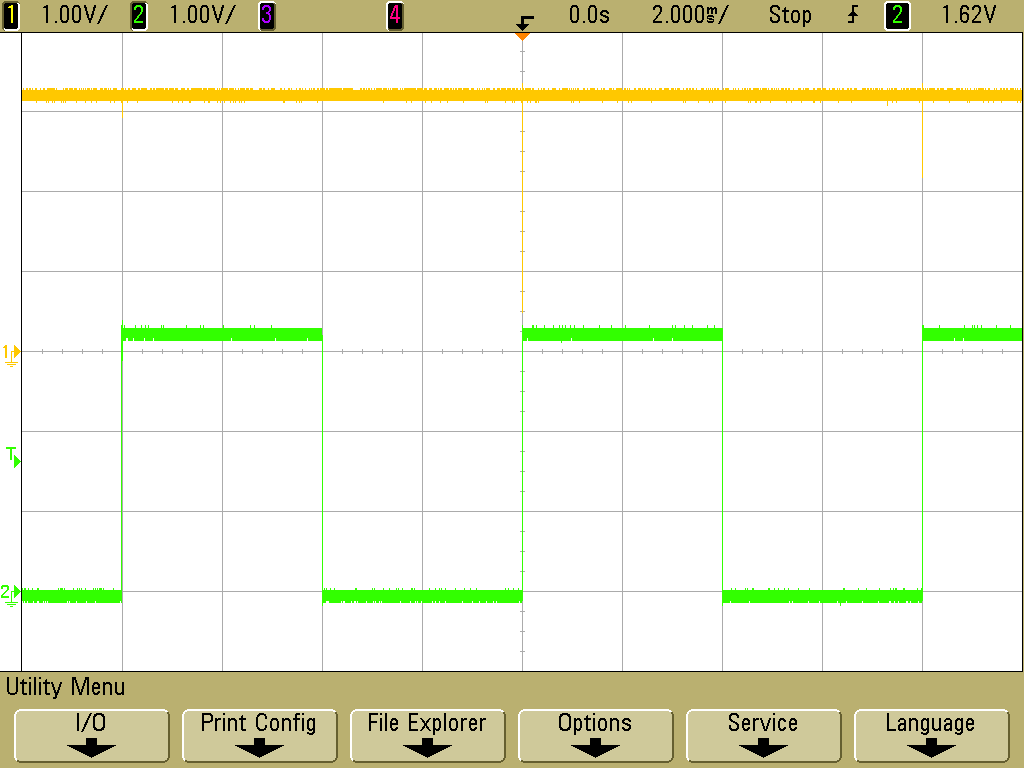
\includegraphics[width=0.8\textwidth]{figures/scope/ctrl_signal_test_1_scope/print_00.png}
  \caption{Control signals \texttt{nRES} and \texttt{nTX} during reset and integration phases.}
  \label{fig:ctrl_test1}
\end{figure}

% ---- FIGURE: control signal test 2 ----
% Files: figures/scope/ctrl_signal_test_2_scope/print_02.png
%        figures/scope/ctrl_signal_test_2_scope/print_03.png
%        figures/scope/ctrl_signal_test_2_scope/print_04.png
% Suggested caption: "Extended view showing multiple successive scan cycles. The periodic reset pulse is visible at the start of each cycle."
\begin{figure}[h]
  \centering
  % 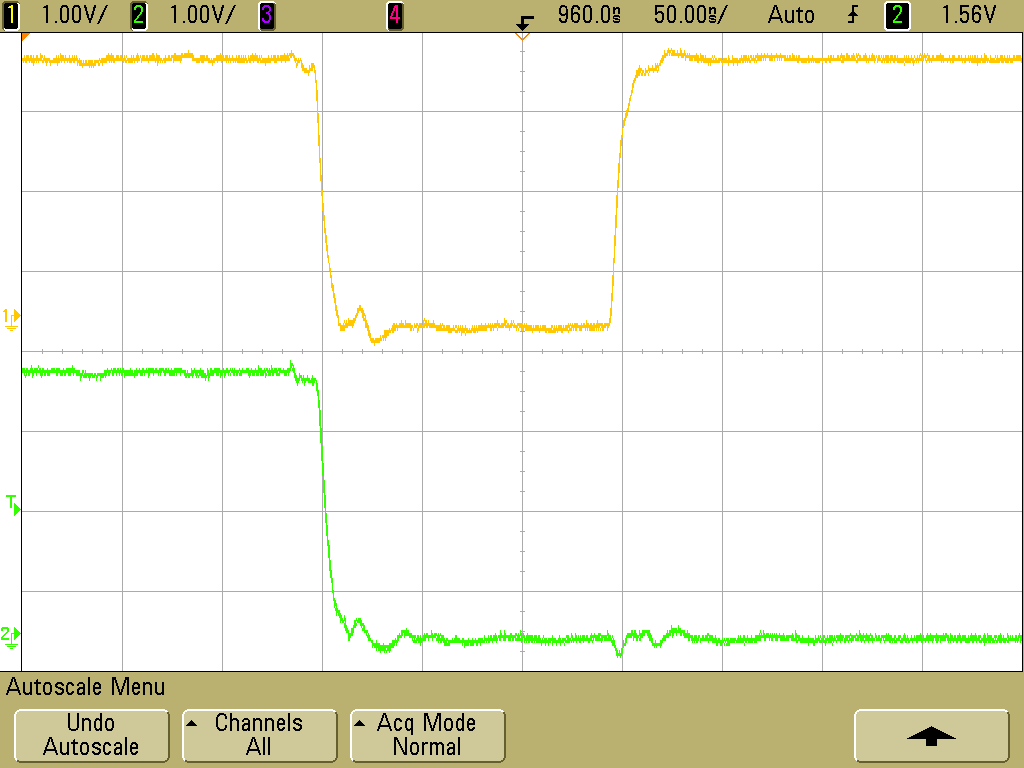
\includegraphics[width=0.8\textwidth]{figures/scope/ctrl_signal_test_2_scope/print_02.png}
  \caption{Successive scan cycles showing periodic \texttt{nRES} pulses.}
  \label{fig:ctrl_test2}
\end{figure}

\subsection{Readout Timing Verification}

The address bug signals \texttt{AX} and \texttt{AY} were measured during the READOUT state to verify that the FSM stepped through all pixel addresses in the correct order and held each address for the configured dwell time.

% ---- FIGURE: AX/AY address stepping ----
% Files: figures/scope/readout_ax_ay_test_1_scope/ax.png
%        figures/scope/readout_ax_ay_test_1_scope/ay.png
% Suggested caption: "AX[2:0] and AY[2:0] address bus signals during
%   full-frame READOUT. AX steps 0–7 for each row; AY increments after every eighth pixel."
\begin{figure}[h]
  \centering
  % 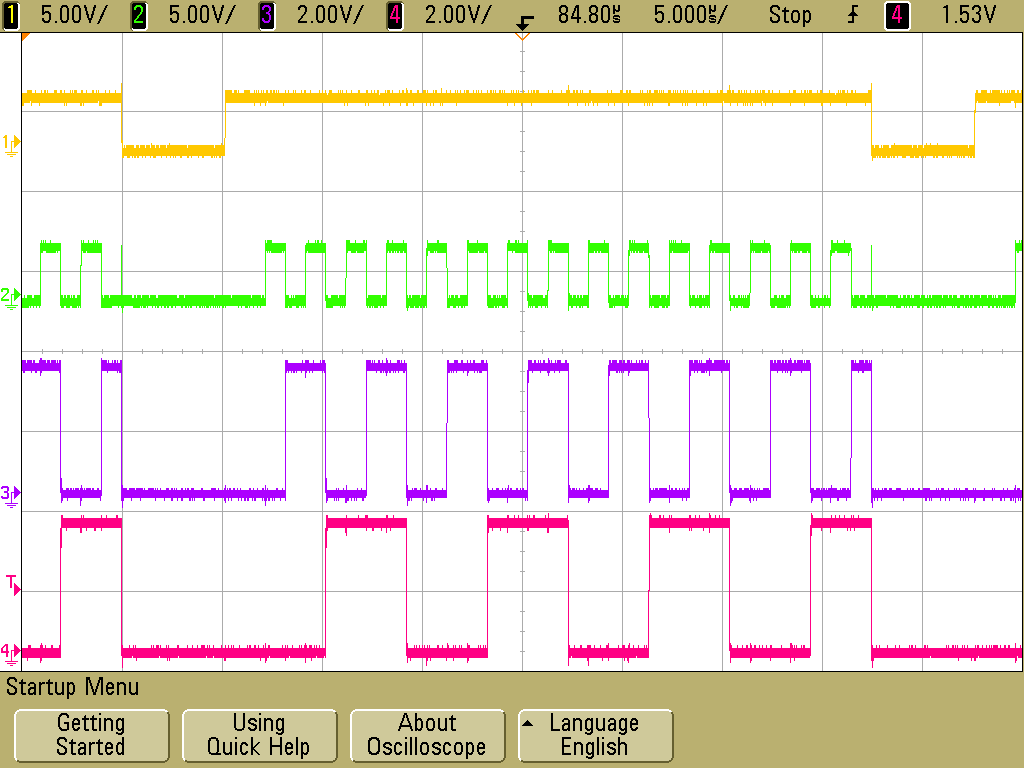
\includegraphics[width=0.48\textwidth]{figures/scope/readout_ax_ay_test_1_scope/ax.png}
  % 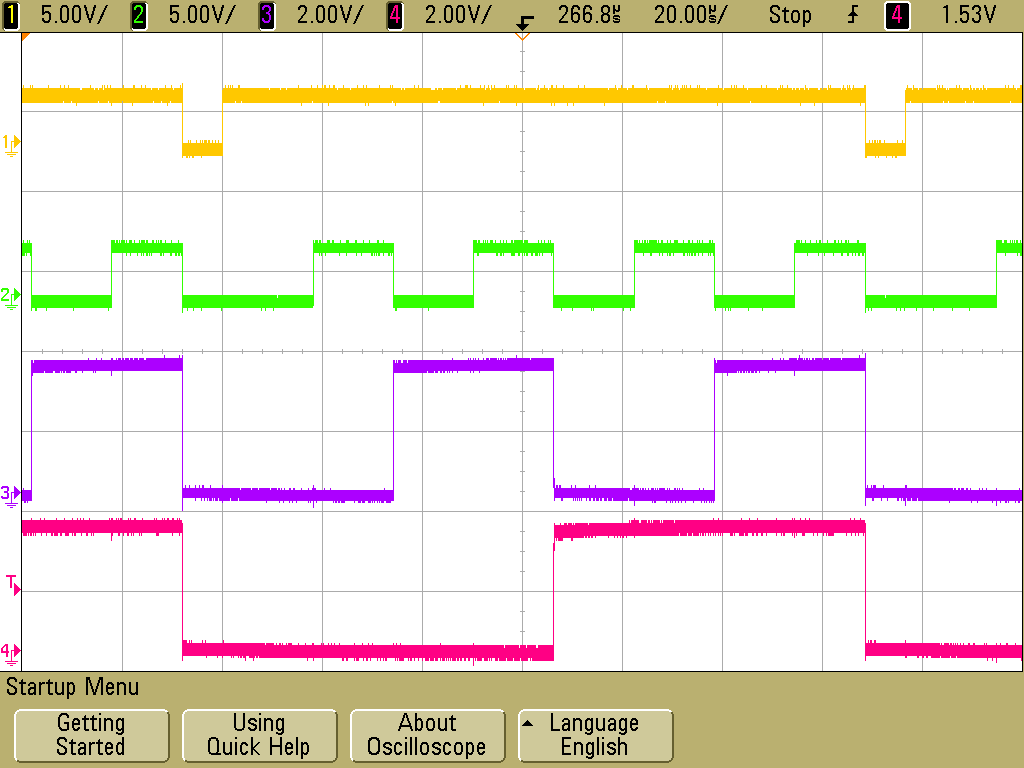
\includegraphics[width=0.48\textwidth]{figures/scope/readout_ax_ay_test_1_scope/ay.png}
  \caption{\texttt{AX} (left) and \texttt{AY} (right) address signals during a full 8$\times$8 readout scan.}
  \label{fig:ax_ay}
\end{figure}

% ---- FIGURE: readout signal tests ----
% Files: figures/scope/readout_signal_test_1_scope/print_09.png  (overview)
%        figures/scope/readout_signal_test_1_scope/print_10.png
%        figures/scope/readout_signal_test_1_scope/print_11.png
%        figures/scope/readout_signal_test_1_scope/print_12.png
% Suggested caption: "Full readout waveform: nRES, nTX, and the AX bus cross one complete scan. The dwell period between address transitions is visible as flat regions on the AX trace."
\begin{figure}[htbp]
  \centering
  % 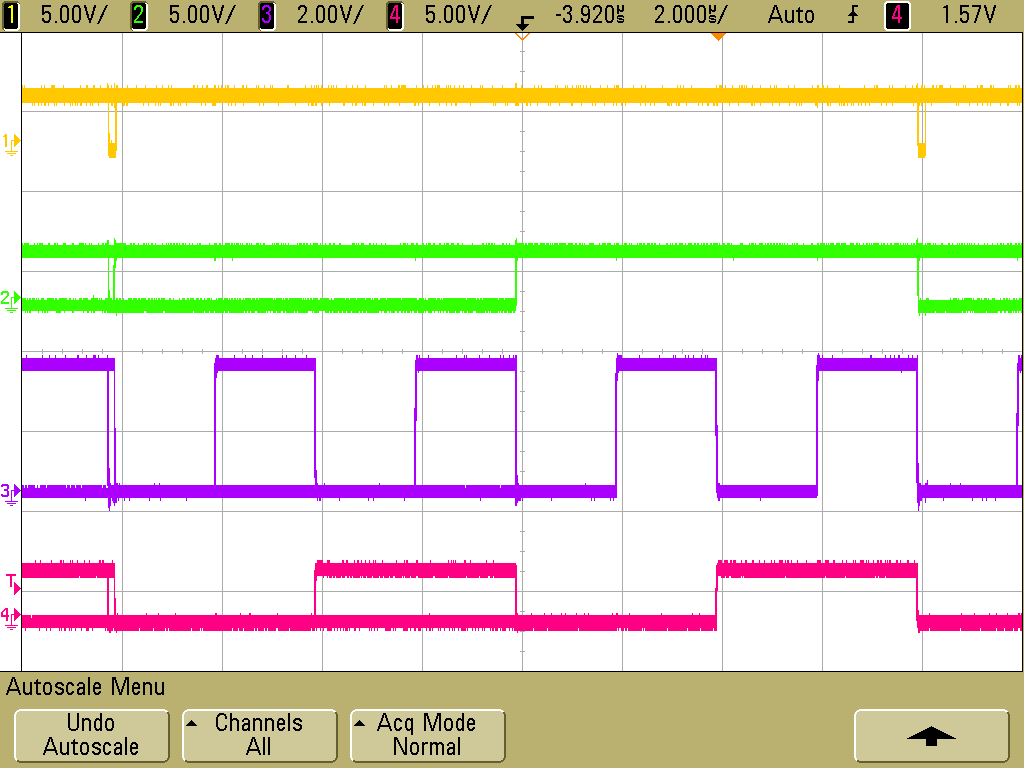
\includegraphics[width=0.8\textwidth]{figures/scope/readout_signal_test_1_scope/print_09.png}
  \caption{Full readout cycle waveform showing \texttt{nRES},
    \texttt{nTX}, and the \texttt{AX} address bus.}
  \label{fig:readout_full}
\end{figure}

% ---- FIGURE: readout signal tests 4 and 5 (detailed dwell) ----
% Files: figures/scope/readout_signal_test_4_scope/ax/print_02.png
%        figures/scope/readout_signal_test_4_scope/ax/print_03.png
%        figures/scope/readout_signal_test_4_scope/ay/print_00.png
%        figures/scope/readout_signal_test_4_scope/ay/print_01.png
%        figures/scope/readout_signal_test_5_scope/ax/print_04.png
%        figures/scope/readout_signal_test_5_scope/ax/print_05.png
%        figures/scope/readout_signal_test_5_scope/print_06.png
%        figures/scope/readout_signal_test_5_scope/print_07.png
% Suggested caption: "Zoomed view of AX transitions showing the dwell period between consecutive pixel addresses. The flat region width corresponds to the configured dwell_us value."

\subsection{Pixel Data Acquisition}

After confirming the correct timing, the pixel ADC values were read over UART and compared against oscilloscope measurements of the sensor analog output voltage.

% ---- FIGURE: pixel value measurements ----
% Files: figures/scope/pixel_values/measure1/print_11.png
%        figures/scope/pixel_values/measure1/print_12.png
%        figures/scope/pixel_values/measure2/print_13.png
%        figures/scope/pixel_values/measure3/print_14.png  (through print_17.png)
% Suggested caption: "Sensor analog output voltage at XADC VAUX0 during
%   pixel readout. The voltage steps correspond to successive pixel
%   addresses. The ADC-reported value for each pixel is annotated."
\begin{figure}[h]
  \centering
  % 
\includegraphics[width=0.8\textwidth]{figures/scope/pixel_values/measure1/print_11.png}
  \caption{Sensor analog output voltage during readout, showing
    pixel-to-pixel voltage variation. ADC values read back over UART correspond to the measured voltages.}
  \label{fig:pixel_values}
\end{figure}

% TODO: add a table comparing oscilloscope-measured voltages against UART-readback ADC values for a representative set of pixels. Formula: voltage = ADC_value / 4096 * 1.0 V (XADC reference)